\documentclass[tikz, margin=3mm]{standalone}
\usetikzlibrary{positioning, shapes}

\begin{document}
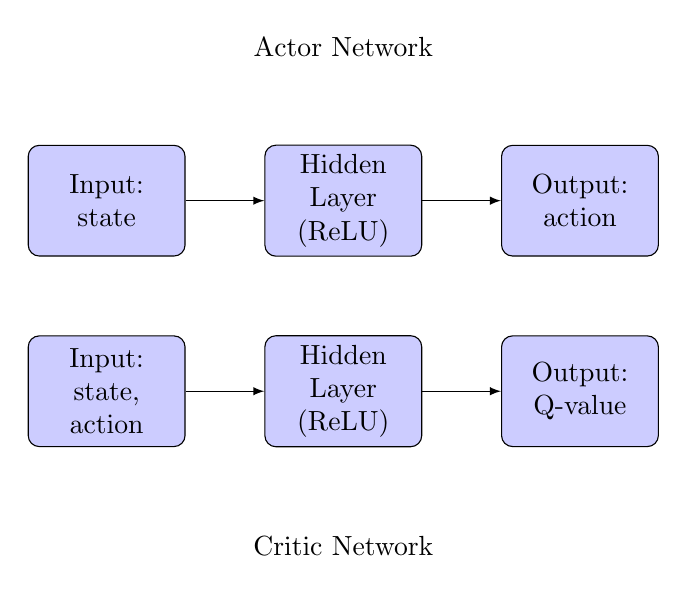
\begin{tikzpicture}[
    node distance=1cm and 1cm,
    block/.style={rectangle, draw, fill=blue!20, text width=5em, text centered, rounded corners, minimum height=4em},
    line/.style={draw, -latex}
]
    % Actor network
    \node [block] (input1) {Input: state};
    \node [block, right=of input1] (hidden1) {Hidden Layer (ReLU)};
    \node [block, right=of hidden1] (output1) {Output: action};

    % Critic network
    \node [block, below=of input1] (input2) {Input: state, action};
    \node [block, right=of input2] (hidden2) {Hidden Layer (ReLU)};
    \node [block, right=of hidden2] (output2) {Output: Q-value};

    % Paths
    \path [line] (input1) -- (hidden1);
    \path [line] (hidden1) -- (output1);
    \path [line] (input2) -- (hidden2);
    \path [line] (hidden2) -- (output2);

    % Labels
    \node [above=of hidden1, align=center] {Actor Network};
    \node [below=of hidden2, align=center] {Critic Network};
\end{tikzpicture}
\end{document}
